\section{Sensorer} \label{sec:sensorer}
I det tiltænkte system benyttes forskellige sensorer, hvorfra systemet skal agere. Herunder benyttes elektroder til opsamling af EMG-signaler. Til målingen af EMG-signaler ønskes en repræsentation af energimængden i signalet. For at dette opnås skal systemet passere en envalope filtrering. Yderligere ønskes at kunne justere forstærkningen, for at kune tilpasse amplituden af EMG-signalet, og dermed gøre systemet mere nuanceret. Den justerebare forstærkning vil tillade ALS-patienter at få forstærkeret signalet i takt med at det progressive muskelsvind. 

\subsection{Elektromyografi}
Til behandling af EMG-signalet, anvendes Muscle Sensor V3, der fremover vil bliver refereret som 'EMG-forstærker'. Denne komponent måler en differens af de elektriske potentialer der måles gennem elektroderne. EMG-forstærkeren overholder de opstillede krav, og kan anvendes direkte med mikrokontrolleren. EMG-forstærkeren består af en intrumenteringsforstærker, et passivt højpasfilter, en full-wave rectifier, et aktivt lavpass filter og en justerbar forstærker \citep{advancertech2013}. 

Et illustration af hvordan EMG-forstærkeren behandler et målt signal ses af \autoref{fig:sinussignal}.
\begin{figure}[H]
\centering
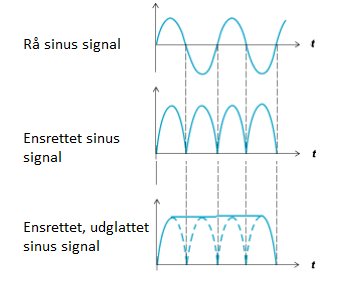
\includegraphics[width=0.8\textwidth]{figures/sinussignal.png}
\caption{Tre sinus signaler. Henholdsvis et råt sinus signal, ensrettet sinus signal og ensrettet samt udglattet sinus signal \citep{advancertech2013}.}
\label{fig:sinussignal}
\end{figure}

Med udgangspunkt i \autoref{fig:sinussignal} ses signalet som sinus kurven. Hertil passerer det højpasfilteret der dæmper dc støjen og dermed offsettet i signalet. Dette ses som signalet sinuskurven der svinger omkring 0, og er nøvendig for at ensretningen viker efter hensigten. Dernæst ensrettes signalet, således at de negative værdier inverteres, og at der kun er svingninger i positiv retning. Dernæst fortages et envalope af signalet, og ses som det udglattede signalet, hvortil der er beregnet en knækfrekvens på $1,94~Hz$, ud fra \autoref{eq:lavcutfre}. 

\begin{equation}\label{eq:lavcutfre}
f_c = \frac{1}{2 \pi C R} = \frac{1}{2 \pi*1*10^{-6}F*80,6*10^3\Omega} = 1,94~Hz
\end{equation}

EMG-forstærkeren har en minimum spændingsforsyning på $\pm 3~V$ samt en maksimal spændingsforsyning på $\pm 30~V$. Herudover er der mulighed for at justere gain fra 0,002 gange - 20,700 gange \citep{advancertech2013}. 



%Synes ikke det passer ind her? Er det ikke meningen dette skal være mere overordnet, og så specificerer vi os senere til hvordan vi vil måle, sådan til vores forsøg?
%Den ene elektrode placeres over enten rectus femoris eller vastus intermedius (sidder under rectus femoris) og den anden elektrode placeres over biceps femoris. Reference elektroden placeres ved??.. 


%\subsection{Accelerometer}
%Et accelerometer er en elektromekanisk enhed, som både kan måle statiske eller dynamiske accerlerationskræfter. De statiske kræfter kan være tyngdekraften, hvortil det er muligt at bestemme orienteringen af accelerometeret i forhold til jorden. De dynamiske kræfter såsom bevægelse, stød og vibrationer, gør det muligt at analysere accelerometeres bevægelse samt hastighed. 
%ADXL335Z er et 3-aksialt accelerometer, som har et arbejdsområde på minimum $\pm$ 3 g. Hertil arbejdes der ved dette accelerometer med analoge output signaler proportionelle med accelerationen \citep{analogdevices2010}. 

%\textbf{Tilføj noget om sensitivitet og evt. illustration af g-påvirking og udregning af vinkel skal tilføjes hertil.}

%Støj kan reduceres ved at placere en 0.1 mikro f capacitor i nærheden, det er dog nødvendigt at tilføje mere, hvis der er 50 KHz støj, da det vil kunne resultere i fejl i accelerations målingen. Støjens tæthed vil forminskes i takt med at forsyningsspændingen forøges.
%Fase sensitiv demodulation teknikker er anvendt for at bestemme magnituden samt accelerationens retning. Demodulator outputtet er forstærket og bragt igennem en 32 k ohm modstand. – noget med det forebygger aliasing 
%  - Jeg ser dette som 'ligegyldigt' nu, da det handler om kondensator og støj. Kan ikke se hvorfor det skal bruges (endnu) måske skal det bruges efter vi har lavet pilotforsøg, hvis der viser sig meget støj





